\documentclass{acm_proc_article-sp}
%\documentclass[conference]{IEEEtran} - For IEEE, search for [@IEEE] tags
% Add the compsoc option for Computer Society conferences.
%
% If IEEEtran.cls has not been installed into the LaTeX system files,
% manually specify the path to it like:
% \documentclass[conference]{../sty/IEEEtran}

% Some very useful LaTeX packages include:
% (uncomment the ones you want to load)

%
\usepackage{graphicx}
\usepackage[lined,boxed,commentsnumbered]{algorithm2e}
%\usepackage{draftwatermark}


% correct bad hyphenation here
\hyphenation{op-tical net-works semi-conduc-tor sche-dul-ing}


\begin{document}
%

\title{Using Fractal Clustering to explore Behavioral Correlation for
reducing energy consumption in Sensor Networks}

% author names and affiliations
% use a multiple column layout for up to three different
% affiliations
% \author{\IEEEauthorblockN{Fernando Rodrigues}
% \IEEEauthorblockA{University of Fortaleza\\Fortaleza - Ceara - Brazil\\
% fernandorodrigues@edu.unifor.br}
% \and
% \IEEEauthorblockN{Angelo Brayner}
% \IEEEauthorblockA{University of Fortaleza\\
% Fortaleza - Ceara - Brazil\\
% brayner@unifor.br}
% \and
% \IEEEauthorblockN{Jose E. Bessa Maia}
% \IEEEauthorblockA{State University of Ceara\\
% Fortaleza - Ceara - Brazil\\
% jose.maia@uece.br}}


% make the title area
\maketitle


\begin{abstract}

Sensor clustering is an efficient strategy to reduce the number of messages
transmitted to the sink in a multi-hop Wireless Sensor Network.
In this work, we present a new approach to cluster sensors in WSN, denoted
Behavioral Correlation in WSN (BCWSN), based on the behave of recent historical
data collected by sensors. Instead of using the spatial distance among sensors
for clustering them, the proposed approach uses the concept of behavioral
correlation to group sensors, that takes into account the concepts of difference
in magnitude and trend of sensed data. For clusters maintenance, we propose
an alternative approach based on Fractal Clustering, where this technique use
the concept of Fractal Dimension to find the best configuration for clusters
based on the Minimum Difference of Fractal Dimension strategy.
Furthermore, Cluster Head (CH) technique is used as scheduling intra-clustering
method.
We develop a framework to address several important technical challenges,
including how to partition the sensors into clusters (using Behavioral
Correlation), how to dynamically maintain the clusters in response to
environmental changes (using Fractal Clustering), how to schedule the sensors in
a cluster (CH) and how to explore temporal correlation for restore the data in
the sink with high fidelity (using Linear Regression with threshold error),
apart from dealing with multiple types of sensed data at the same time.
To the best of our knowledge, there is no other paper that uses Fractal
Clustering to maintain clusters while making predictions about multiple types of
sensed data simultaneously in a WSN.
In order to validate our approach, simulations with a prototype have been
conducted over real data. The results show that, with 5\% error threshold in
temporal prediction, BCWSN can save the communication overhead up to 98.95\%
over naive strategy and 90.4\% over a temporal correlation approach, while the
RMSE remains roughly stable.

% The results point to gains of up to 97.72\% over naive strategy in terms of
% reduction in message transmission and 45,12\% of reduction in data sensing,
% while the RMSE remains roughly stable. To the best of our knowledge, we believe
% that our proposal brings gains in energy efficiency for WSNs.

% The best way to improve prediction accuracy is by decreasing prediction errors,
% using the same energy amount than the second version, but there is a trade-off
% between prediction accuracy and energy consumption.

\end{abstract}

% IEEEtran.cls defaults to using nonbold math in the Abstract.
% This preserves the distinction between vectors and scalars. However,
% if the conference you are submitting to favors bold math in the abstract,
% then you can use LaTeX's standard command \boldmath at the very start
% of the abstract to achieve this. Many IEEE journals/conferences frown on
% math in the abstract anyway.

% no keywords




% For peer review papers, you can put extra information on the cover
% page as needed:
% \ifCLASSOPTIONpeerreview
% \begin{center} \bfseries EDICS Category: 3-BBND \end{center}
% \fi
%
% For peerreview papers, this IEEEtran command inserts a page break and
% creates the second title. It will be ignored for other modes.
%\IEEEpeerreviewmaketitle - [@IEEE]



\section{Introduction}
% no \IEEEPARstart


Sensors are devices used to collect data from the environment related to the
detection or measurement of physical phenomena. Sensors are limited in power,
computational capacity, and memory. Advances in wireless communication have
enabled the development of massive-scale wireless sensor networks (WSNs). In a
WSN, sensors are usually scattered in the network and use low-power
communication channels. Thus, sensors disseminate collected data to a base
station, from where the information (query) was originally requested. Wireless
sensor networks (WSNs) have been widely used for environmental monitoring (e.g.,
traffic, habitat), industrial sensing and diagnostics (e.g., factory, supply
chains), infrastructure protection (e.g., water distribution), battlefield
awareness (e.g., multi-target tracking) and context-aware computing (e.g.,
intelligent home) applications.

In spite of advances in WSN technology, a critical key point is still the
energy consumption of sensor nodes. It is well known that communication among
sensors is the activity responsible for the bulk of the power consumption. By
reducing communication costs, energy may be drastically saved, consequently
increasing the WSN's lifetime. An effective strategy to reduce energy
consumption is thus to reduce the number of messages (sensed data) sent across
the network. Nevertheless, the less the number of sensed data is transmitted,
the lower the accuracy of results provided by a WSN. Thus higher accuracy in
WSNs comes at a higher energy cost.

By now, it is well-known that data collected by WSN are strongly temporally
and/or spatial correlated \cite{Yoon2005, Chu2006}. The traditional spatial data
correlation is related to the idea that the physical proximity among sensors
leads to similar measurements (values) of sensed data, phenomenon known as
"principle of spatial locality". Thus, one can infer that from the capture of
some sensors readings (located in some regions of sensing space), it is possible
to obtain, approximately, the values of the readings of other sensors in its
surroundings. On the other hand, the temporal correlation indicates the various
readings of a sensor within a time interval have a certain approximation of
their values (principle of temporal locality). Such a feature makes possible to
predict (with a certain margin of error) sensed values in the future based on
data collected in the past.

% Grouping sensors in clusters is the main technique used to take advantage of the
% principle of spatial locality for reducing the energy consumption in WSNs. This
% is because one can use only a few representative nodes from each cluster to
% sense data in a given spatial region (cluster) in which sensors are spatially
% correlated.
% Several works have been proposed in order to use that technique, with different
% approaches \cite{Chu2006, Villas2012, Singh2010, Liu2007, Shah2007}.

Nonetheless, in several scenarios, sensors which are not spatially close to each
other may have similar data reading patterns. In order to illustrate such a
claim, consider a dense WSN deployed to monitor forest fires. 
Now, suppose a scenario in which the monitored region is affected by dozens of
small forest fires. Figure \ref{fig:contour_lines} depicts a possible temperature
contour lines graph for this hypothetical situation. Observe that the contour
lines in Figure \ref{fig:contour_lines} form several closed regions representing
areas which may have small forest fire areas, where it is very likely that the
temperature measurements of sensors in those spatially separated regions present
high correlation. For that reason, we claim that in such cases, a better
alternative would be to use sensor clustering strategy based on
\textit{Behavioral Correlation}.

The idea behind the concept of {\it Behavioral Correlation} is to identify
similar patterns of sensor readings even in sensors which are geographically
distant from each other. Thus, one could apply a Behavioral Correlation
Clustering (BCC) technique to group sensors which are spatially separated into a
single cluster, in contrast to existing spatio-temporal correlation techniques.
The BCC technique clusters sensors for which the forecasting models of sensed
data time series are approximately the same independent of spatial proximity of
sensors.

\begin{figure}[!htb]
\centering
	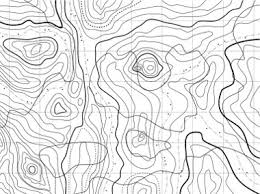
\includegraphics[scale=0.9]{I2.png}
    \caption{Contours lines of temperature}
    \label{fig:contour_lines}
\end{figure}

Furthermore, to make the maintenance of clusters, we have developed a technique
based on Fractal Clustering \cite{Barbara1999}, which uses the Minimum
Difference Fractal Dimension (MDFD), where sensors that send new data
(novelties) are allocated by the sink node in cluster where the smallest change
in value of Fractal Dimension occurs, making the choice of the new most
appropriate node's cluster (with new data readings received by sink node) the
most accurate possible.

In this sense, this paper presents a new approach for clustering sensors in
WSNs. The main features of the proposed approach are: {\it (i)} Cluster
formation based on the \textit{Behavioral Correlation} of the sensors, which, in
turn, is computed from the time series of sensor readings by applying a
\textit{Similarity Measure}; {\it (ii)} Maintenance of clusters through a
technique called Fractal Clustering, where the values of Fractal Dimension of
each cluster are used to maintain the structure of the clusters, and; {\it
(iii)} the use of a linear regression model for the temporal suppression of
sensed data, through the maximum error level (threshold) desired by the user, is
used to control the data to be sent to the sink. Hence, sensor nodes
only transmit data which are novelties for the regression model applied by our
proposal. Furthermore, Cluster Head technique have been implemented to select
node (scheduling one sensor - CH - in each cluster) responsible for aggregating
the data collected by all sensors, coordinating the operation of such a cluster.


The remainder of this document is organized as follows. Section
\ref{related-work} describes related work and point out the differences between
our method and existing methods. In Section \ref{implementing-bcwsn} the
proposed Behavioral Correlation in WSN (BCWSN) method and the sensor-scheduling
policy are presented and discussed. Simulations with a Sinalgo prototype
operating over real sensor data are reported in Section \ref{eval}. Finally,
Section \ref{conclusion} concludes the paper.


\section{Related Work}
\label{related-work}

% In \cite{Vuran2004}, the authors propose a strategy to cluster sensors in WSNs.
% The idea is the following: given a set of N sensors, M nodes, with $M < N$, are
% chosen to send data. The M representative nodes are defined based on the
% application of a distortion function ($D(M)$) on sensed data.
% The spatial distance between the nodes (representative) directly influences the
% computation of the distortion function by means of a correlation coefficient.
% That work does not take into account the energy capacity of each node as a
% criterion for choosing representative nodes, although this is a very important
% factor due to the restrictive characteristics regarding the energy consumption
% of the nodes in a WSN.

In EAST \cite{Villas2012}, sensors are grouped into two levels, under a spatial
correlation approach, while the leader and the representative nodes perform a
temporal suppression technique.
The leader node generates a representative value for each cluster based on data
received by the representative nodes, which form a subset of all the nodes that
sense the same event. The sensed area is divided into "event areas", which in
turn are divided into "correlation regions (c) or cells", where the formers will
be managed, each one, for a "Coordinator node" and the "correlation areas" will
be represented, one by one, by a "Representative node" because a single reading
within this region is enough to represent it.
The size of the correlation region (c) can be decremented or incremented by the
sink according to the application and the characteristics of the event, to
maintain the accuracy of the data collected. However, in this approach, clusters
are formed exclusively by spatial criterion, i.e. the Euclidean distance between
sensors.

Another way to group sensor nodes into clusters is through measures of
dissimilarity.
In EEDC \cite{Liu2007}, such measures of dissimilarity are calculated by the
sink node for pairs of nodes of the network, according to the maximum distance
between them.
So, the measure of dissimilarity between two nodes is calculated based on up to
$3$ parameters, namely:
the differences in magnitude (\textit{M}) and trend (\textit{T}) of the data
values and the geographical/euclidean distance between nodes ($g_{max}dist$).
The criterion of formation of clusters is based on the maximum threshold of
dissimilarity (max\_dst) defined by a tuple (\textit{M}, \textit{T},
$g_{max}dist$), based on the measure of dissimilarity between the nodes. It
works as follows: $1)$ Initially, the sensed data by each node are sent in the
form of a temporal series for the sink. $2)$ The sink then stores all the data
from the sensors and then calculates the measure of dissimilarity (previously
mentioned) for each pair of nodes of the network. $3)$ With the measures
calculated and the maximum threshold of dissimilarity (max\_dst), the sink
divides the nodes into clusters. 
That work does not takes into account the energy reserve of each node as a
criterion for choosing representative nodes (it is used an algorithm that makes,
simultaneously, the equitable scheduling - round robin - along with the random
choice of representatives nodes). In this work, we choose Representative Nodes /
Cluster Heads according to the remaining energy level and the minimum distance
to the sink. Moreover, unlike \cite{Liu2007}, we took into account readings from
multiple different data types by sensors.

The spatial correlation through the formation of clusters is addressed in
\cite{Pham2010} as a flooding algorithm where the sink node starts to
send messages to the other nodes of the network, inviting them to form groups
from criteria such as a dissimilarity measure, in addition to the physical
proximity between nodes, since, of course, the message forwarding in a WSN
occurs between adjacent nodes (i.e. geographically close). Cluster Heads (CHs)
are selected, basically, by 2 parameters: {\it (i)} the nodes that are one hop
from the ancestor that sent the message calculate the measure of dissimilarity
with the mean value informed in the message and then those that are within the
threshold of dissimilarity if they apply for CH, where {\it (ii)} it is said to
be the CH the one that have higher level of energy reserve.
We should notice that, during the process of forming clusters, the nodes that
will form the communication backbone between each Cluster Head node and the sink
are also configured. A scheduling of each cluster is done through round robin in
order to decide which member node that will be active in each time slot making
the sensing and sending the data to its respective CH.
The weak point is the process of forming clusters, in
which there is an intensive exchange of messages, scattering a significant
amount of energy from the network sensors.

% In \cite{Shah2007}, the spatial correlation is explored by a mechanism called
% the GSC (Gridiron Spatial Correlation), where the sensed region has a Cluster
% Head that will be in the center of the region delimited by r (radius of the
% monitored region), which will be divided into correlated regular regions
% (quadratic), according to the spatial density level chosen, defined through
% $\theta$ (size of the correlation region equal to $\theta^2$). In this way,
% active sensors will be chosen according to 2 basic parameters: {\it (i)} the
% proximity of the them regarding the center of the regions correlated and {\it
% (ii)} their energy level must be within a certain threshold, above the ones of
% their closest neighbours. The scheduling of active nodes works through the
% passage of a list by the cluster-head for all nodes with the nodes being active
% in each time slot, where this configuration is only changed when one of the
% active nodes has its energy level below the threshold established.
% That work does not describe how the energy threshold is calculated neither how
% this reconfiguration of the sizes of the rectangles are done and not even gives
% examples of that.

Carvalho \textit{et al.} \cite{Carvalho2011} proposed applying Multivariate
Spatio-Temporal Correlation to improving prediction accuracy in a WSN. But the
major drawback of this work is that it do not reduces the energy consumption of
the network compared to other existing approaches. In fact, it even increases
the energy consumption of the network in many situations. In our work, using
multiple linear regression together with fractal clustering, we achieved reduce
the overall energy consumption of the network, obtaining results with a Root
Mean Square Error (RMSE) for the prediction data (w.r.t. the sensed data) even
smaller than other approaches.

In Fractal Clustering \cite{Barbara2000}, the authors explain how to use the
\textit{Fractal Dimension} to cluster datasets, from an initialization step
based on the nearest neighbor strategy, that create the initial clusters. Then
they present the algorithm of the incremental step, which uses \textit{Fractal
Dimension} calculation based on an implementation of Box Counting algorithm,
called FD3 \cite{Liebovitch1989}. In our proposal, we use an adapted version of
this algorithm (Fractal Clustering) for the maintenance of clusters each time a
change in the sensed environment is detected and reported to the sink node by
some sensor in the network.

\section{Implementing Behavioral Correlation in WSNs}
\label{implementing-bcwsn}

In this section, we present the proposed approach for clustering sensors in a
WSN based on the notion of {\it Behavioral Correlation}. Our approach, called
Behavioral Correlation in Wireless Sensor Networks (\textit{BCWSN} for short),
is based on clustering sensors initially by means of behavioral correlation
(described in \ref{clustering-sensors}) between gathered variables (such as
temperature, humidity and light), which in turn is computed from the time series
of sensor readings, and, after the first clusters were formed, \textit{Fractal
Clustering} method is used in cluster maintenance (\ref{cluster-maintenance}).
Clustering reduces the traffic on the network, since the Cluster Heads
coordinate the data flow (messaging) between sensors and the sink.
Furthermore, a linear regression model is used for the temporal suppression
(prediction) of data to be sent from each sensor to the sink node.

% Two different approaches for intra-cluster sensor node scheduling have been
% implemented in order to uniformly distribute the sensing activity for the
% sensor nodes of a cluster. In the first one, called Representative Nodes (RNs),
% only one node in each cluster $C_{i}$ is chosen at each time to represent that
% cluster. In other words, a Representative Node is responsible for sensing and
% predicting data in $C_{i}$ for given time interval. In this case, we have a
% greater energy economy in the network as a trade-off from a little
% general precision, because changes in sensed fenomena at network positions where
% the sensors are in stand-by mode (non-Representative Nodes) would not be
% captured. To stand up to this weakness, we have a second method, called
% Cluster Heads (CHs). In this other approach, on the other hand, one sensor node
% (the CH) in each cluster $C_{i}$ is selected to coordinate the data sensing
% activity carried out by all nodes in $C_{i}$. So, changes are promptly sensed by
% active nodes, having major impact on energy expediture from nodes activation.

\subsection{The BCWSN Mechanism}


The algorithm BCWSN can be divided into five steps described next.


\subsubsection{Learning Stage}

In this step, the sink node collects sensed data from all sensors belonging to
the network in order to compute the initial cluster formation and the
coefficients of the linear regression equation (see Section \ref
{data-predict}). Thus, the sink node firstly sends a broadcast message to all
nodes of the network, requesting the following data from sensors:
battery level, spatial location and sensed values. The amount of data used by the
learning stage is a parameter, denoted initial slot time, which should be
defined by the application expert (e.g. 70). Each sensor answers the broadcast
message from sink in a batch mode, i.e., it makes all sensing tasks required and
sends only one message response to sink node with all reading data.


\subsubsection{Clustering Sensor Nodes}
\label{clustering-sensors}

As already mentioned, the BCWSN mechanism clusters sensor nodes by means of
behavioral correlation. In order to compute behavioral correlation, a
\textit{similarity measure} \cite{Liu2007} is used. Thus, sensors with similar
data reading pattern for all sensed data type are grouped into a single cluster.
The similarity measure among sensed data of two different sensors is defined by 
similarity of magnitude and similarity of trend, defined next.

\newtheorem{defini}{Definition}

\begin{defini}
Similarity of magnitude-M: Two sensors ($S$ and $S'$) with time series
$S$=\{$s_{1}$,$s_{2}$,\ldots,$s_{n}$\} and
$S'$ = \{$s'_{1}$,$s'_{2}$,\ldots,$s'_{n}$\} are magnitude-M similar if 
\begin{equation}
\label{equ:magni}
\frac{\sum_{i=1}^{n} |s_{i}-s'_{i}|}{n} \leq M
\end{equation}
%$\displaystyle \sum_{i = 0}^{n} |s_{1_i}-s_{2_i}| \leq M$
\end{defini}

\begin{defini}
Similarity of trend-T: Two sensors ($S$ and $S'$) with time series
$S$=\{$s_{1}$,$s_{2}$,\ldots,$s_{n}$\} and
$S'$=\{$s'_{1}$,$s'_{2}$,\ldots,$s'_{n}$\} are trend-T similar if 
\begin{equation}
\label{equ:trend}
\frac{P}{n} \geq T,
\end{equation}
where $n$ is the total number of sensed data and $P$ is the number of pairs
$(s_{i},s'_{i})$ in the time series which satisfy $\nabla s_{i} \times \nabla
s'_{i} \geq 0$, where $\nabla s_{i} = s_{i} - s_{i-1}$, $\nabla
s'_{i} = s'_{i} - s'_{i-1}$ and $1 < i \leq n$.
\end{defini}

Thus, sensors which are magnitude-M and trend-T similar for all sensed data
type, they are grouped in the same cluster. After all time series of all sensors
in a WSN have been processed during the learning phase, the initial WSN cluster
configuration is defined by the sink.

Once the sensors are initially grouped into clusters, the cluster head of each
cluster is defined by applying the energy level criterion.
In other words, for each cluster, the cluster head is the node with the highest
energy level. In the case of nodes with same energy level, the node with the
shortest distance to the sink node is chosen.


\subsubsection{In-Network Data Prediction}
\label{data-predict}

The in-network prediction implemented by BCWSN relies on the
following linear regression equation, applied for each sensed data type:
$\hat{S}(t) = a + bt$.
The time $t$ is an independent variable. $\hat{S}(t)$ represents the estimated
value of $S(t)$ and is variable with $t$. Parameter $a$ is the interceptor-t
(value of $\hat{S}(t)$ for $t=0$) and $b$ is the stretch slope, and are computed
as follows:
\begin{equation}
	a = \frac{1}{N}\left(\sum S_{i} - b\sum t_{i} \right) = \bar{S} - b\bar{t},
\end{equation}
\vspace*{-.3cm}
\begin{equation}
	b = \frac{\sum \left(t_{i} - \bar{t}\right)\left(S_{i} - \bar{S}\right)}{\sum \left(t_{i} - \bar{t}\right)^{2}}.
\end{equation}

The idea behind this method is that both the sink and the sensor node know the
regression equations to predict the sensed values for all sensed data. Thus, a
sensor node does not need to send any data to sink, since it is able to predict
all sensed data by the sensors. Thus, the network is saving power of sensors
\cite{MaiaACR2013}.

During the Learning Stage, the sink node computes the initial coefficients $a$
and $b$ for each sensed data type, for each sensor node, based on the time
series received from them. Thereafter, the sink node sends the calculated
coefficients to the respective sensors.

 
\subsubsection{Sensing}

% As already mentioned, two different approaches for intra-cluster sensor node
% scheduling have been implemented in order to uniformly distribute the sensing
% activity for the sensor nodes of a cluster. In the first one, called
% Representative Node (RN), only one node in a cluster $C_{i}$ is responsible
% for sensing and predicting data in $C_{i}$ for given time interval. In the
% second method, called Cluster Heads (CHs), on the other hand, one sensor node
% (the CH) in each cluster $C_{i}$ is selected to coordinate the data sensing
% activity carried out by all nodes in $C_{i}$.

As already mentioned, one sensor node (Cluster Head) in each cluster $C_{i}$ is
selected to coordinate the data sensing activity carried out by all nodes in
$C_{i}$.

After a node receives the corresponding coefficients, it starts using these
coefficients in reading / prediction loop.
Whenever a sensor node senses values \{$v_{1}$,$v_{2}$, \ldots,$v_{n}$\} of
certain data type \{$d_{1}$,$d_{2}$,\ldots,$d_{n}$\}, it verifies if anyone of
$v_{n}$ is not within a ``tolerable difference'' $t$, i.e., $v_{n} \not \in
[p_{n}-t,p_{n}+t], t \geq 0$, where $p_{n}$ is the predicted value by applying
the regression equation corresponding to data type $d_{n}$. Any data outside the
tolerable difference are treated as novelty for the model.
The ``tolerable difference'' is a parameter, set by the application expert (e.g.
$5\%$ or $10\%$).

% In RN mode, only the representative nodes (one for cluster) receive the
% coefficients and execute the reading / prediction loop. Whenever a representative
% node detects a given amount of novelties $n$ (defined by the application
% expert), it should send the novelties to the sink for updating the predicting
% model by computing new regression coefficients.

% In CH mode, all sensors in a cluster receive their respective coefficients and
% execute the reading / prediction loop. 

When a sensor node $s$ detects a given amount of novelties $n$ (Sensor Delay,
defined by the application expert), it sends the novelties as a notification to
the Cluster Head of the cluster to which $s$ belongs. The Cluster Head in turn
logs the number of notifications, in such way that when the number of received
notifications is greater than a preset limit $m$ (Cluster Delay, also
defined by the application expert), the CH sends a message to the sink for
computing new regression coefficients for that cluster.

[PAREI AQUI!]

\subsubsection{Cluster Maintenance}
\label{cluster-maintenance}

In the proposed approach, the sink has the ability to automatically and
autonomously maintain the clusters. There are two strategies implemented by
BCWSN to recompute clusters. One strategy is to maintain the sensor clusters
according to the Minimum Difference of Fractal Dimension (MDFD), based on the
Fractal Clustering algorithm (\textit{FC} for short) that allows only
merge operations. The other strategy is according to the Similarity
Measures algorithm (\textit{SM}) that allows split and merge operations.

Let $R_{new}$ be the new reading data to be treated by the sink; let $S_{R}$ be
the sensor which report that ``novelties'' (i.e. new reading - $R_{new}$) to the
sink node; let $C_i$ be the $i-th$ sensor cluster, formed by a 
CH and other cluster members (0 or more sensors); let $D(C_i)$
be the data (sensor's data) of cluster $C_i$; let $D'(C_i)$ denote the data of
cluster $C_i$ with the new reading data $R_{new}$ (i.e. $D'(C_i) = D(C_i) \cup
R_{new}$) and let $F_{d}(D(C_i))$ be the value of Fractal Dimension of the data
of cluster $C_i$.

When \textit{FC} is chosen, in clustering sensor nodes phase (Section
\ref{clustering-sensors}), the Fractal Dimension is calculated and stored for
each initial cluster ($F_{d}(D(C_i)), \forall i$). The idea is to find out which
cluster $C_{\hat{i}}$ the inclusion of new sensor data $R_{new}$ will take the
slightest change in its Fractal Dimension.

The Minimum Difference of Fractal Dimension (MDFD) strategy is as follows:
whenever the sink receives "novelties", i.e. new data ($R_{new}$), from a RN or CH on
a given cluster $C_j$, it calculates which cluster $C_i$ has the minimal
\textit{fractal impact}, i.e. the minimum absolute difference between the
previous Fractal Dimension value (calculated before the new data arrives)
($F_d(D(C_i))$) and the new one ($F_d(D'(C_i))$), where: $D'(C_i) = D(C_i) \cup
R_{new}, \forall i$.
If this minimal difference ($|F_d(D'(C_{\hat{i}})) - F_d(D(C_{\hat{i}}))|$,
where $\hat{i} = min(|F_d(D'(C_i)) - F_d(D(C_i))|), \forall i$), is greater than
a certain threshold ($\tau$) - defined by the application expert (e.g. $\tau =
0.03$), then this new data $R_{new}$ is simply rejected as noise.
On the other hand, if the cluster $C_i$ is the same $C_j$ (i.e. $i=j$), the
sink just add the new data $R_{new}$ to the corresponding sensor in this cluster.
Otherwise, the sink must remove this sensor node ($S_{R}$ with new data
$R_{new}$) from its old cluster $C_j$ and add it to the new cluster $(C_i)$.
The Algorithm \ref{alg:MDFD} outlines this strategy.

\begin{algorithm}
 \SetAlgoLined
 \LinesNumbered
 \KwData{input parameters: set of all K current sensor clusters (\{$C_i \vert 1
 \leq i \leq K$\}), values of Fractal Dimension of all current sensor clusters
 ($F_d(D(C_i))$), sensor node($S_{R}$) with new data ($R_{new}$)}
 \KwResult{processes Fractal Clustering}
 Sink Node receives new data ($R_{new}$) from sensor ($S_{R}$) of cluster $C_j$\;
 \For{i = 1 \ldots K}{
	  Compute $F_d(D(C_i))$\;
	  Let $D'(C_i) = D(C_i) \cup R_{new}$\;
	  Compute $F_d(D'(C_i))$\;
 }
  Find $\hat{i} = min(|F_d(D'(C_i)) - F_d(D(C_i))|)$\;
  \eIf{$|F_d(D'(C_{\hat{i}})) - F_d(D(C_{\hat{i}}))| > \tau$}{
  	Discard $R_{new}$ as noise\;
  }{
  	\eIf{$j \neq \hat{i}$}{
  		Remove $S_{R}$ from cluster $C_j$\;
  		Place $S_{R}$ in cluster $C_\hat{i}$\;
  	}{
    	Replace $S_{R}$ in cluster $C_\hat{i}$\;
    }
  }
 
 \caption{Fractal Clustering Algorithm - FC Strategy}
 \label{alg:MDFD}
\end{algorithm}

% the sensor nodes in $c$ are not
% meeting the minimum similarity requirements M-magnitude and T-trend anymore. In
% that case, the sink disjoins $c$ in two or more new clusters, selecting new
% representative nodes or cluster heads (one for each of the new clusters) based
% on the criteria described in Section \ref{clustering-sensors}.

On the other hand, the strategy using \textit{SM} for Cluster Maintenance can be
subdivided into two phases: splitting and merging clusters. Splitting cluster is
the following:
Whenever the sink receives "novelties" (new data) from a RN or CH on a given
cluster $C$, it checks if the sensor nodes in $C$ are not meeting the minimum
similarity requirements M-magnitude and T-trend anymore. In that case, the sink
disjoins $C$ in two or more new clusters, selecting new representative nodes or
cluster heads (one for each of the new clusters) based on the criteria described
in Section \ref{clustering-sensors}.

For merging clusters, the sink monitors the number of sensors in each cluster of
the network. This way, whenever there are a large number of cluster splits and
the cluster rate occupation is lower than a limit defined by the application
expert, the sink triggers a global process for merging clusters. Thus, the
proposed approach avoids the existence of clusters composed by a very low number
of sensors. Such a feature is quite important, since after several cluster
splits in a network, one could have clusters with only one sensor node.

\section{Empirical Evaluation}
\label{eval}

In order to show the potentials of the proposed approach, simulations over real
data have been conducted and the main results achieved so far are presented and
discussed in this section. Thus, in this section, we first describe how the
simulation prototype has been set up. Thereafter, the empirical results are
quantitatively presented and qualitatively discussed.

\subsection{Implementation}
\label{implementation}

A simulation prototype was implemented in Java, exploiting the facilities
provided by Sinalgo \cite{Sinalgo2007}, a well-known framework for testing and
validating network algorithms. The simulations have been executed on i7 computer
with 8 GB RAM and Mac OS X as operating system.
One of the main reasons for choosing Sinalgo is because it is very scalable in
nature, allowing that simulations with up to several thousands of sensor nodes
be executed in a reasonable time. The data used for the simulation were
extracted from the real data of experiment Intel Lab Data \cite{Intel2004}. 

\subsection{Simulation Setup}
\label{data-and-experiments}

M-magnitude parameter has been configured with the value of $1.5$ and T-trend
was $5\%$, the same as the error threshold (t). The amount of initial data sensing
(initial slot time) was 70 readings, used for the learning stage.

The performance evaluation was done through four application versions, which we
used to simulate and compare multiple linear regression to simple linear
regression and to the original version of a monitoring application. This
monitoring application simulates the gathering of two variables from the
environment: ``temperature'' and/or ``humidity'', according to kind of test.
%[The application versions to achieve the simulations are]
In the experiments, we have executed the following approaches: {\it
  (i)} Naive approach \cite{Madden2005}, where all nodes send their sensed
data to the sink node;  {\it
  (ii)} Adaga-P* approach \cite{MaiaACR2013} \cite{MaiaSAC2013}, which
implicitly implements spatial correlation to cluster sensors and exploits the
benefits of using a linear regression model to reduce the number of messages
injected into the network;  {\it
  (iii)} BCWSN-SM-RN approach, where, after the formation of the clusters based on the
\textit{Behavioral Correlation}, only the Representative Node (RN) of each
cluster senses data and the clusters are maintained by \textit{SM}
strategy, and;  {\it 
  (iv)} BCWSN-FC-CH approach, which implements the BCWSN, with the scheduling
policy of Cluster Heads (CH) and the maintenance of clusters through the
\textit{FC} strategy.

In order to compare the aforementioned approaches, three metrics have been
deployed: 1) The Root Mean Square Error (RMSE) to verify the accuracy of
approach; 2) The Number of Messages injected into the network, which is a
critical factor to measure energy consumption of the network, and; 3) The
Number of Sensed Data, which impacts in the network energy consumption and in
the accuracy of the result provided by each approach. The RMSE is calculated by
reference to the naive approach filtered values.

It is important to note that the BCWSN-SM-CH and BCWSN-FC-RN approaches were
disregarded because unsatisfactory results were found. That is due to the fact
that: {\it
  (i)} BCWSN-SM-CH approach, the \textit{SM} strategy was less effective than
  \textit{FC} strategy when all sensors are sensing (CH), causing the [worst]
  sensor clustering increases the RMS Error, while it increases the total number of
  messages and sensor readings too, and; {\it
  (ii)} BCWSN-FC-RN approach, the \textit{FC} strategy makes the total number of
  clusters decrease over time, decreasing the RN (sensors that make readings)
  too. So, the RMS Error increases as well.

The simulation parameters are presented in Table \ref{tab:parameters}.

\begin{table}[h!]
\caption{Simulation parameters}
\label{tab:parameters}
\begin{center}
\begin{tabular}{|l||l|}
\hline
Parameters &Values\\
\hline\hline
Sink node &1 (center) \\
\hline
\# of nodes &54 \\
\hline
\# of cycles executed &10000 \\
\hline
Notification rate (per second) &31 \\
\hline
Sensed data type &Temp. / Hum. \\
\hline
Initial slot time (\# learning stage) &70 \\
\hline
M-magnitude &1.5 \\
\hline
T-trend &0.05 \\
\hline
Tolerable difference {\it(t)} &0.05 \\
\hline
Sensor delay {\it(n)} &(1, 5) \\
\hline
Limit per cluster {\it(m)} &(1, 5) \\
\hline
FC threshold ($\tau$) &0.03 \\
\hline
\end{tabular}
\end{center}
\end{table}


\subsection{Results and Discussion}
\label{results-and-discussion}

% Table \ref{tab:rmseVsRounds} presents the RMSE values of the four approaches
% evaluated during the experiments, in the following cycles (rounds): 100, 500,
% 1000 and 10000; with Sensed type = T, Sensor delay {\it(n)} = 1 and Limit per
% cluster {\it(m)} = 1.

% \begin{table}[h!]
% \caption{RMSE vs. Rounds}
% \label{tab:rmseVsRounds}
% \begin{center}
% \begin{tabular}{|l||l|l|l|l|}
% \hline
% RMSE &100 &500 &1000 &10000 \\
% \hline\hline
% Naive &0 &0 &0 &0 \\
% \hline
% Adaga-P* &0.299 &0.414 &0.465 &0.502 \\
% \hline
% BCWSN-SM-RN &0.897 &0.499 &0.51 &0.534 \\
% \hline
% BCWSN-FC-CH &0.235 &0.4 &0.369 &0.378 \\
% \hline
% \end{tabular}
% \end{center}
% \end{table}

% In Table \ref{tab:numMsgVsRounds}, we present the total Number of Messages (Num Msg)
% of the four approaches evaluated, in the following cycles (rounds): 100, 500,
% 1000 and 10000; with Sensed type = T, Sensor delay {\it(n)} = 1 and Limit per
% cluster {\it(m)} = 1.
% 
% \begin{table}[h!]
% \caption{Number of Messages vs. Rounds}
% \label{tab:numMsgVsRounds}
% \begin{center}
% \begin{tabular}{|l||l|l|l|l|}
% \hline
% Num Msg &100 &500 &1000 &10000 \\
% \hline\hline
% Naive &20417 &110017 &222017 &2182038 \\
% \hline
% Adaga-P* &4089 &14146 &25918 &266250 \\
% \hline
% BCWSN-SM-RN &509 &3640 &7928 &96197 \\
% \hline
% BCWSN-FC-CH &605 &2205 &2891 &8361 \\
% \hline
% \end{tabular}
% \end{center}
% \end{table}

% Table \ref{tab:sensReadVsRounds} shows, for cycles (rounds): 100, 500, 1000 and
% 10000; with Sensed type = T, Sensor delay {\it(n)} = 1 and Limit per cluster
% {\it(m)} = 1, the total Number of Sensed Data (Sensor Reading) from all sensors
% of the network.
% 
% \begin{table}[h!]
% \caption{Number of Sensed Data vs. Rounds}
% \label{tab:sensReadVsRounds}
% \begin{center}
% \begin{tabular}{|l||l|l|l|l|}
% \hline
% Sensor Reading &100 &500 &1000 &10000 \\
% \hline\hline
% Naive &5112 &26312 &52812 &521809 \\
% \hline
% Adaga-P* &5114 &26314 &52814 &521811 \\
% \hline
% BCWSN-SM-RN &3785 &14554 &27533 &271617 \\
% \hline
% BCWSN-FC-CH &3795 &11927 &16147 &46503 \\
% \hline
% \end{tabular}
% \end{center}
% \end{table}


Table \ref{tab:rmse} presents the average (AVG), standard deviation (STD),
maximum (MAX) and minimum (MIN) value for the RMSE of the four approaches
evaluated during the experiments.

\begin{table}[h!]
\caption{RMSE per Round (1000 cycles)}
\label{tab:rmse}
\begin{center}
\begin{tabular}{|l||l|l|l|l|}
\hline
RMSE &AVG &STD &MAX &MIN \\
\hline\hline
Naive &0 &0 &0 &0 \\
\hline
Adaga-P* &0.4251 &0.0328 &0.47 &0.299 \\
\hline
BCWSN-SM-RN &0.5387 &0.0649 &0.897 &0.499 \\
\hline
BCWSN-FC-CH &0.3963 &0.0386 &0.69 &0.229 \\
\hline
\end{tabular}
\end{center}
\end{table}


Looking more closely to Table \ref{tab:rmse}, one can observe that BCWSN-SM-RN
presented a RMSE of $0.5$ (with average $0.5387$ and standard deviation $0.0649$),
while the average of transmitted messages is $96.25\%$ smaller than the Naive
approach (Table \ref{tab:num-msg}). Compared to Adaga-P*, the average of
messages exchanged in BCWSN-SM-RN is $65.61\%$ lower and the average of sensed
data is $49.94\%$ lower. The RMSE produced by BCWSN-SM-RN is $26.72\%$ higher in
average than the RMSE presented by Adaga-P*.
% $96.25\%$ = ((224 - 8.39)*100)/224
% $65.61\%$ = ((24.4 - 8.39)*100)/24.4
% $49.94\%$ = ((53 - 26.53)*100)/53
% $26.72\%$ = ((0.5387 - 0.4251)*100)/0.4251

Regarding BCWSN-FC-CH approach, although the average RMSE is $0.3963$ (whereas
in Naive approach it is virtually $0$), the average of number of exchanged
messages is $98.95\%$ lower than Naive, besides the number of data readings
$75.85\%$ lower in average. When compared to Adaga-P*, the average RMSE of
BCWSN-FC-CH approach is $6.77\%$ ($0.0288$) smaller, while the average of number
of messages is $90.4\%$ smaller. It is worthwhile to note that we have
considered the both directions of transmission, i.e. from and into sensor nodes,
for computing communication cost.
% and the number of exchanged messages $75.85\%$ smaller in average.

% $0.0288$ = 0.4251 - 0.3963
% $98.95\%$ = ((224 - 2.34)*100)/224
% $75.85\%$ = ((53 - 12.8)*100)/53


\begin{table}[h!]
\caption{Number of Messages per Round (1000 cycles)}
\label{tab:num-msg}
\begin{center}
\begin{tabular}{|l||l|l|l|l|}
\hline
Num Msg &AVG &STD &MAX &MIN \\
\hline\hline
Naive &224 &0 &224 &224 \\
\hline
Adaga-P* &24.40 &14.09 &109 &0 \\
\hline
BCWSN-SM-RN &8.39 &9.45 &55 &0 \\
\hline
BCWSN-FC-CH &2.34 &4.15 &33 &0 \\
\hline
\end{tabular}
\end{center}
\end{table}

In Table \ref{tab:num-msg}, the values for column MIN for Adaga-P*, BCWSN-SM-RN
and BCWSN-FC-CH are equal to zero because in several rounds the predict value is
equal to the sensed value. In this case, the sensor does not need to forward the
sensed value. In Table \ref{tab:sens-read}, the values for column MIN for
BCWSN-SM-RN and BCWSN-FC-CH are equal to 0(zero) due to the cluster split or
merge process, during which the sensors stop to sense. 
The average of number of messages and sensor readings in BCWSN-FC-CH approach is
lower than in BCWSN-SM-RN, because the number of clusters decreases over time in
Fractal Clustering strategy, while in Similarity Measures, there are constantly
cluster splits, only with a merge process when the number of clusters exceeds a
threshold.

In BCWSN-SM-RN, the only sensors that constantly sensing are the representative
nodes, but, in some situations as during a merge process, all the nodes are
sensing, while in others, none of them is active because everyone are waiting
for new coefficients from sink node.
So, the Standard Deviation of number of message and sensor reading is greater
than in BCWSN-FC-CH.


\begin{table}[h!]
\caption{Sensed data per Round (1000 cycles)}
\label{tab:sens-read}
\begin{center}
\begin{tabular}{|l||l|l|l|l|}
\hline
Sensor Reading &AVG &STD &MAX &MIN \\
\hline\hline
Naive &53 &0 &53 &53 \\
\hline
Adaga-P* &53 &0 &53 &53 \\
\hline
BCWSN-SM-RN &26.53 &19.20 &53 &0 \\
\hline
BCWSN-FC-CH &12.80 &10.30 &53 &0 \\
\hline
\end{tabular}
\end{center}
\end{table}


Figure \ref{fig:rmse} depicts the evolution of RMSE per round. The RMSE in the
BCWSN-SM-RN and Adaga-P* approaches tend to get very close to $0.5$ at about $1000$
cycles, while the BCWSN-FC-CH stabilizes at about $0.37$ in the same point. Thus,
BCWSN-FC-CH provides a good compromise between accuracy and reduction in energy
consumption, since it reduces the communication activity and data readings (see
Tables \ref{tab:num-msg} and \ref{tab:sens-read}). It is important to note that
in the Naive approach, the RMSE is always 0 (zero), because all sensors send all
sensed data to the sink.

\begin{figure}[!htb]
\centering
	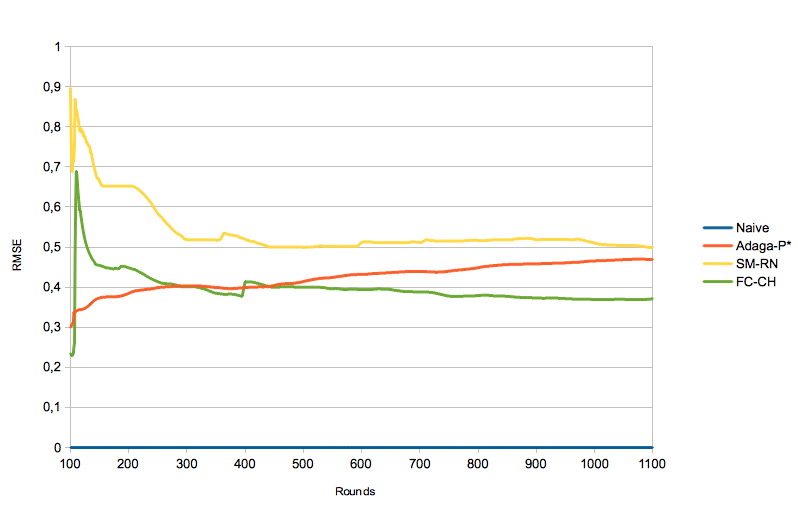
\includegraphics[scale=0.33]{WsneeFD_RMSE.png}
    \caption{RMSE per Round}
    \label{fig:rmse}
\end{figure}

One can identify a peak in Figure \ref{fig:rmse} for the BCWSN-SM-RN and
BCWSN-FC-CH curves. The reason for this is due to the fact that the initial
cluster formation is only an initialization step for the two approaches.
Since all sensors stay sensing in the BCWSN-FC-CH approach, the RMSE peak is
lower than in BCWSN-SM-RN, where only representative nodes are responsible for
sensing data and there is only one representative node per cluster.
%the number of sensed data is small as well.
Thus the BCWSN accuracy is jeopardized at the beginning. Nonetheless, the
BCWSN-SM-RN and BCWSN-FC-CH approaches are able to dynamically adjust the
accuracy by reducing the RMSE.

In Figure \ref{fig:num-msg}, one can observe the number of transmitted messages
per round. In the Naive approach, the number of messages is steady, since in
each round all sensors send sensed data to the sink. It is important to observe
that, in average, BCWSN-FC-CH and BCWSN-SM-RN transmit less messages than Adaga-P*
(see Table \ref{tab:num-msg}). However, there are some peaks in BCWSN-SM-RN
curve, which represent periods in time when clusters are being restructured
(splitting or merging), since the clusters, in this approach, are always
undergoing division and, at times, go through the merge process. This can be
proved by the high standard deviation for this approach in Table
\ref{tab:num-msg}.

\begin{figure}[!htb]
\begin{center}
	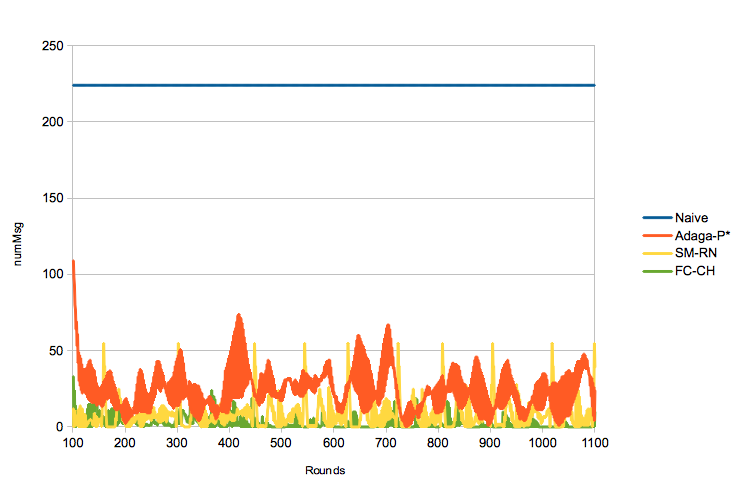
\includegraphics[scale=0.35]{WsneeFD_NumMsgPerRound.png}
    \caption{Number of Messages per Round}
    \label{fig:num-msg}
\end{center}
\end{figure}


Finally, Figure \ref{fig:sens-reading} shows the evolution of the amount of
sensed data for the four evaluated approaches.
Naive and Adaga-P* approaches, as one can observe, have the same number of
sensed data (53 per round), because all sensors in those approaches sense data
during all cycles. In BCWSN-FC-CH, sensors do not sense while they are waiting to
receive new coefficients after sending new data to sink (during Fractal
Clustering process). In the case of BCWSN-SM-RN, only representative nodes (one
per cluster) make data reading continuously, but during merge process, all sensors
must sense data, leading reading data peaks.

\begin{figure}[!htb]
\centering
	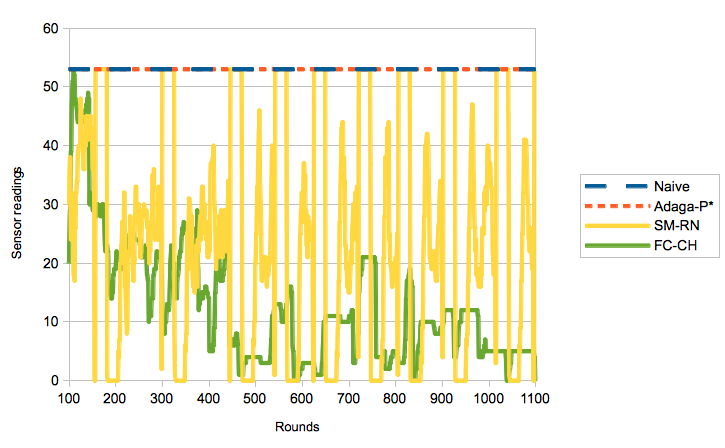
\includegraphics[scale=0.35]{WsneeFD_SReadPerRound.png}
    \caption{Number of Sensed Data per Round}
    \label{fig:sens-reading}
\end{figure}


\section{Conclusion}
\label{conclusion}

In this paper, we have described a new approach for clustering sensors in WSNs
based on the notion of behavioral correlation. Behavioral correlation identifies
sensors with similar data reading patterns, between one or more (different) data
type readings. Moreover, two different approaches to select of active nodes in
each cluster have been proposed: Representative Nodes (RNs) and Cluster Heads
(CHs), besides two strategies for cluster maintenance: Similarity
Measures and Fractal Clustering.

The results presented in Section \ref{results-and-discussion} show that the use
of data behavioral correlation associated with a temporal correlation technique,
associated with a correct strategy for cluster maintenance may significantly
decrease energy consumption in WSNs, while assuring a low RMS Error.

In this work, the similarity among time series behavior has been measured by
applying similarity in magnitude and trend. Now, we are working on evaluating
measures of distance between prediction models to assess the dissimilarity in
sensed data behavior. Moreover, we are evaluation the use of traditional
techniques of data mining, such as K-Means, to perform the initial grouping of
sensors into clusters, overriding the use of similarity measures for such
purpose.


% conference papers do not normally have an appendix



\bibliographystyle{IEEEtran}
\bibliography{IEEEabrv,SAC2015rodrigues_brayner_maia}  
% SAC2015rodrigues_brayner_maia.bib is the name of the Bibliography in this case
% You must have a proper ".bib" file
%  and remember to run:
% latex bibtex latex latex
% to resolve all references

\end{document}